\section{Immersivity and vision}
The first thing that probably comes to mind when talking about 3D and stereoscopy is games and movies. These two happen to be the most popular and money-making mass entertainment media nowadays, apparently carrying forward very different imagery philosophies: cinema was born for telling carefully prefabricated stories, meanwhile a game had interaction at its core and one’s actions would make his own stories. They have actually very much in common, especially regarding how images are percieved or must be percieved by an human observer. Needless to say, they inevitably crossed their paths in a war where each one wanted to be a little more of the other. Games borrowed hollywood-like storytelling while movies experimented with 3D environments. Recently film makers are exploring the possibilities of full 360 degree imagery (Figures \ref{fig:zeropoint_demo} and \ref{fig:starwars_trailer}), while gaming industry is pushing to make interactive virtual reality a solid foundation. Both are today focus on the battle of "immersivity", a term referring to how synthetic content generates mental information in individuals so that it is experienced as close as possible to real.\\
%\captionsetup{margin=2cm}
%\captionsetup{justification=centering}
\begin{figure}
\centering
\begin{subfigure}%{0.49\textwidth}
\centering
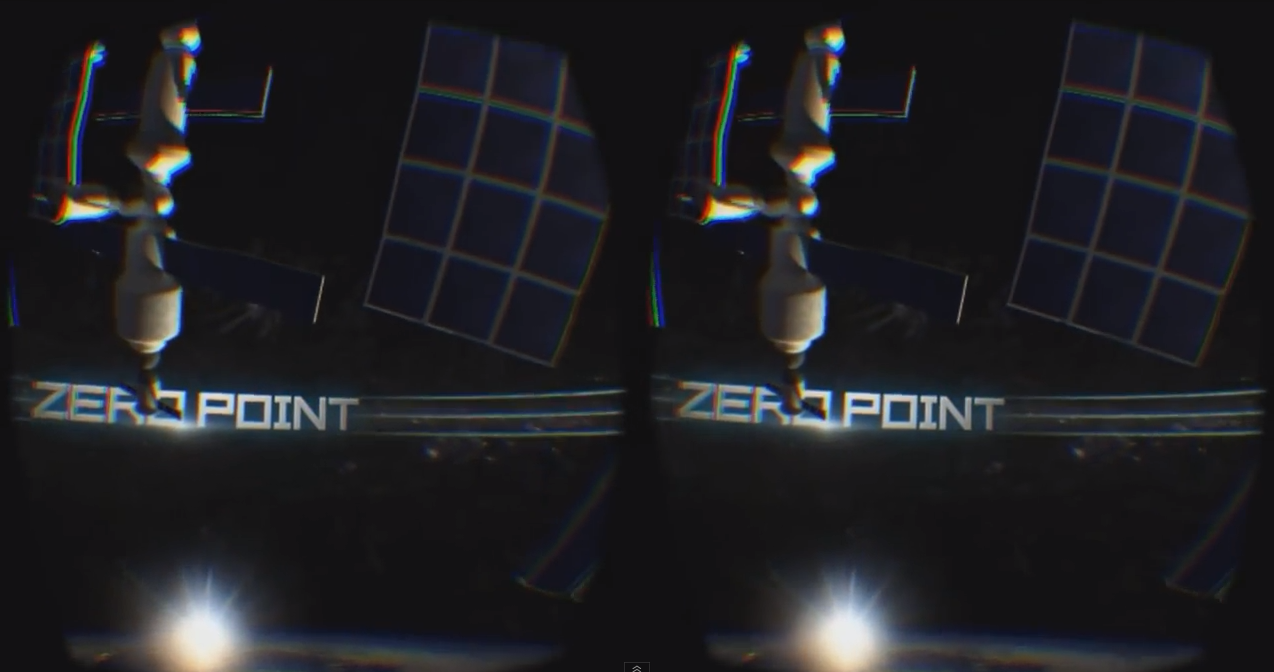
\includegraphics[width=12cm]{pictures/zeropoint_demo.png}
%\caption{This caption is very long \newline ---in fact, it is so long that it doesn't fit on one line}
%\caption
%[1st line \newline 2nd line]
%{\begin{minipage}[t]{.8\linewidth}This is the caption \\This is the second line \end{minipage}}
\caption{Zero Point VR 360 film on Oculus Rift DK2 (source: \href{https://www.youtube.com/watch?v=DsXEUPS2uss}{youtube.com})}
\label{fig:zeropoint_demo}
\end{subfigure}
\vspace{0.5cm}
\begin{subfigure}%{0.49\textwidth}
\centering
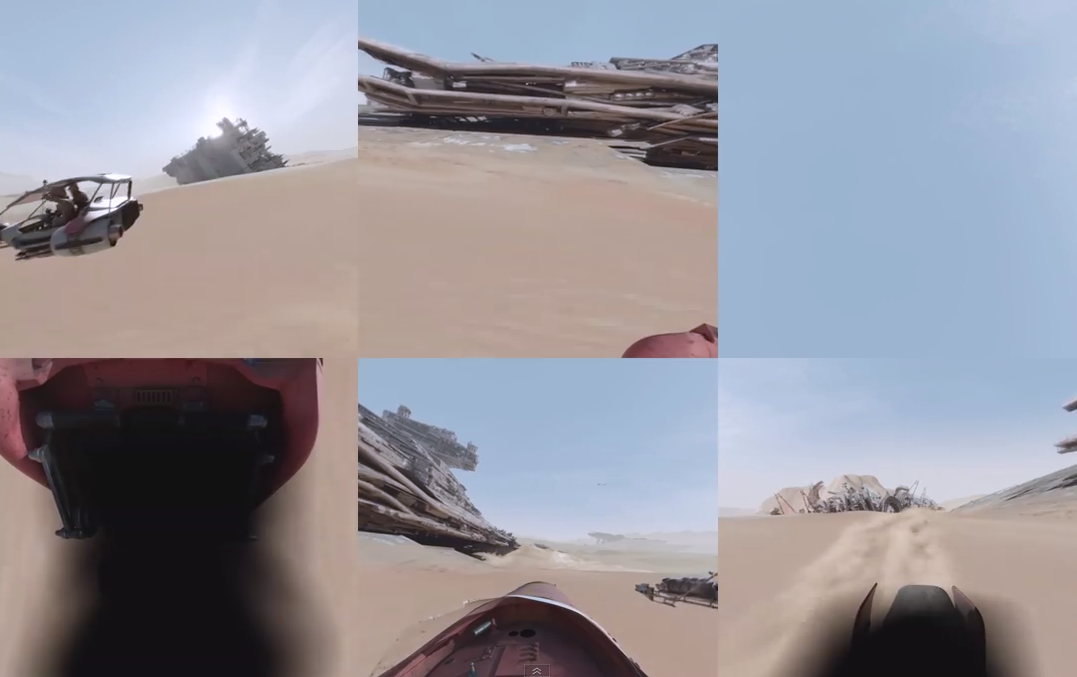
\includegraphics[width=12cm]{pictures/starwars_trailer.png}
%\captionsetup{margin=1cm}
\caption{Star Wars: The Force Awakens Immersive 360 Trailer - different viewpoint screenshots (source: \href{https://www.facebook.com/StarWars/videos/1030579940326940/
}{facebook.com})}
\label{fig:starwars_trailer}
\end{subfigure}
\caption{Two examples of modern union of VR and cinema-like experience}
\label{fig:VR_cinema_examples}
\end{figure}
Current research has been tackling the challenge of what is really immersive and in what ways user experience can be enhanced by means of methods proposed by the previously mentioned doctrines, which stretch from photography and optics to computer graphics and parallel computation. At the same time, the more veteran branch of computer vision has been researching how computationally relevant features can be extracted from real world imagery and put use to it by giving machines comprehension of what is happening around them. Such information can finally support also humans in various tasks where imaging devices are involved, but still computer vision does not focus on better ways to deliver it to end users. Recent marriage of computer vision and virtual reality gave birth to Augmented Reality (AR), a step forward on this matter: target applications would provide more intuitive, interactive and integrated human-machine interfaces, coherently with the world observed.\\
The missing link is where all mentioned features find a place in applications where contact with real world is severed or hijacked and how visual coherence can be enhanced the other way around; the field of studies where human perception is involved can extend its applications from more immersive AR tele-presence to actual artificially improved human perception capabilities. In this work we investigate the challenges of immersive AR by means of a stereoscopic, wide field-of-view (FOV) head-mounted display (HMD) and subsequent realization of see-through with cameras. A custom built stereo camera rig used to achieve stereoscopic images showing in the headset what is directly in front of the user, proposing a way to eventually alter them and/or extract scene information with classic computer vision techniques. Our implementation proposes a uniform way The scenario introduces many real-world effects including latency, optical artefacts, depth perception and other and mismatches in real and virtual content: our implementation proposes a way to uniformly face those problems, by proposing a processing pipeline oriented to be platform independent and easy to experiment with for both human perception and computer vision algorithms.\\
In such attempt, we will traverse common aspects of top-notch techniques for human-computer interaction and perception, belonging to the following fields of expertise:
\begin{itemize}
\item computer vision, which covers the techniques for displaying/enhancing images and extrapolating numerical or symbolic information about the real world. Optics and imaging sensors in general are modelled and therefore used to extract that data, which can range from bare geometrical information (such as distances, position and orientation of a camera or known objects in the scene) to more complex pattern recognition;
\item stereoscopy, a collection of techniques addressing the specific problem of creating or enhancing the illusion of depth in images, exploiting principles in optics and human perception. Most methods involve two separate images to achieve this effect. A combination of such techniques and computer vision models opens the door to computer stereo vision, where more than one image is used to extract data, thus requiring less known parameters from the scene;
\item virtual reality, a discipline that implies mathematical models, actuators and sensors to replicate real world experiences in real time in form of entirely computer-simulated environments and give them interaction capabilities. High relevance is given to human psychology and perception limits in order to recreate a lifelike experience. Images are in this case entirely synthetic: models and image enhancements implied have lot in common with computer vision, although the latter focuses on analysis. We find the most common expression of their combination in what is called augmented reality.
\end{itemize}
In the specific we will experiment with Augmented Reality/Virtuality, with a big focus on high visually immersive applications through the use of a virtual reality headset (referred as HMD, head mounted display). A custom built stereo camera rig is used to achieve stereoscopic images showing in the headset what is directly in front of the user, proposing a way to eventually alter them and/or extract scene information with classic computer vision techniques. The aim is to study the relationship between real world captured and computer generated images and propose an acceptable solution for their blending.

\section{From Augmented reality to Augmented Virtuality}

As we speak of Virtual Reality environments we refer to an experience in which the user is fully immersed, therefore as much isolated from the real world. The perception of one’s self actually being in a different place gets deeper when involving more advanced sensory to track our movements and proxies like avatars to keep alive what is called in VR the "sense of presence", a critical term that expresses the longing deep connection with user perception and psychology [3]. However, there are cases where we might want to take full advantage of the high level of interaction with a virtual environment without giving away the connection with the real world. Virtual reality is mainly meant to bring one’s perception in a controlled environment with its own rules, but what if we want to retain all the aspects of the environment surrounding us plus enhancing it with virtual elements? What if we want indeed to be brought in a different place, where everything is real except our own presence?

Augmented Reality explores ways of including virtual elements in the real world. Typically application’s aim in AR (as we will refer to from now on) span from showing additional information to actually place entire objects in the observed scene. The goal is not only keeping intact contact with reality but making it interactive, enhancing it with arbitrary content in the less obtrusive and more intuitive way possible. AR may or may not have reasons to track user pose or actions, but never involves the usage of avatars of any sort, since user is meant to feel exacly where he actually is.

(image of AR schema)

Nowadays, any device that embeds a camera, a screen and a decent processing unit can feature AR applications, whether Its computational complexity depends on features extraction [4] or no extraction at all [5]. However, even though availability and cost of the hardware makes them accessible to anyyone, their use is not as much diffuse as one would expect. The reason is to find again in obtrusivity and intuitivity, which brings us to transparency and integration. The real seamless integration between real and virtual is limited by the not-as-integration between individuals and devices; current systems are still far from perfect, and system designers typically end up making a number of application dependent trade off, going from simply infographic content such as sport games on tv or HUDs to more immersivity and interaction oriented applications such as medical surgery, complex machinery repair and other tasks that require a specific training.

(image of rugby game on tv with infographic)

On the other hand, some applications are meant exacly for hijacking individual perception, even if not entirely, and carefully control it. That is the case where user is still supposed to interact with reality in some way, but how and when is not up to him. This is the general concept for Mixed Reality (MR), placed midway between pure virtual and real; according to Milgram’s continuum [6], AR is indeed a form of MR in its most reality-oriented form. Moving towards MR we find quite well-known devices such as night or heat vision goggles: not so far away to require avatar representation but enough obtrusive to completely replace environment as we see it.\\
As we start to inject into the scene arbitrary information, which is not at all derived from real environment, we cross the boundary of Augmented Virtuality (AV). Roles are inverted: virtual experience can be somehow enhanced with outside information or content. Usually applications of this kind aim to keep contact with real world but also experiment with new ways of representing it. Also the user feels to be somewhere different from everyday world, but still are cases where avatars are not needed depending on the implementation: think for example to teleoperating a humanoid robot, where an avatar is not really necessary if the robot stays in the sight of the user, even better if his "virtual eyes" are on robots head (figure N). This is not true in a telepresence applications, where real world interaction is mostly percieved as enhanced VR experience.

(Facebook telepresence and titanium strong virtual drift) A very curious but effective example of augmented virtuality. Featured video has been rendered offline but gives a good idea of what is the driver's experience.

\section{Optical and Video See-through devices} %limits and advantages
Devices offering a very good compromise between interactivity and transparency for AR/AV immersive applications are Head Mounted Displays (HMD), where images are projected directly in the user’s view. HMDs often include on-board sensors like gyroscopes and accelerometers or simply passive markers like US or IR to keep track of head position, orientation and speed so that images can be displayed accordingly. As for the displaying part, two systems design have been proposed: video and optical see-through. Both have as image sources real and computer-generated world, but end up to be very different for technical reasons. In a work of Rolland-Fuchs [7] a comprehensive taxonomy of video and optical see-through technology is given, through which we will motivate the choice of our work.

(images from examples of HMDs types)

A video HMD with no images from the real world is common in VR applications: its ability to block out the real world view thus cover the highest user’s field of view with the crispiest computer-generated image possible. Adding on-board image capture capability it can be considered a video see-through device, capable of both AR/AV applications. Experimenting with AV has virtually no limits, since other kind of sensors or even more cameras may be involved to show something different to the user, as soon as a good level of immersion is guaranteed. The same cannot be said for a canonical AR application: captured images should appear as close as real and feel natural to the user, suspending his istinctive disbelief that what he is seeing is not real. A series of optical limits come in play that simply cannot be surpassed by a simple screen, which is just a simplification of how images are percieved by the human eye. To address this lack, the most pursued strategy is providing additional hints to the brain by involving head motion and even eye gaze tracking to act on image behaviour. But even if a good compromise can be reached, it cannot be considered acceptable in the long run: human brain is as good at noticing imperfections as adapting to them. This costant effort generates an increasing amount of stress in the user that, depending on the subject, may experience from simple eye strain to temporary sickness [?].\\
Optical see-through devices sistematically solve the problem, providing semi-transparent lens or screen that lets light in while computer-generated images are merged through a set of mirrors. The connection with reality is kept nearly intact, therefore no perception side-effects are present as soon as device is perfectly calibrated. The limit of optical HMDs is only technological. While they are the best option for AR applications, they still lack the capability of showing environment as only a completely transparent glass would allow or virtual content as only a completely opaque screen would do. Moreover, there is always a discrepancy between overlay (region where virtual and real information are superimposed) and peripheral FOV of the user, an issue video HMD not really have since everything else from the screen is blocked out. Cost and build limits still not allow to cover high field of views such as ones achieved by recent video counterparts like Oculus Rift or Sony VR. In other words, optical see-through solutions are promising for a variety of applications whose working space is within arm reach and require reliability and minimum distraction. Even with the best performance possible, a video see-through headset can be dangerous in situations where seeing what is going on is vital.\\
Optical HMD is so far the candidate to be more present in everyday life in the future. As we already mentioned, its current obtrusive nature makes it hard, but recently a lot of effort has been spent in this direction. "Light" versions of optical HMD can be identified in early commercial products such as Google Glass or the still unreleased Microsoft Hololens (figure N), whose aim is supporting multi-purpose applications to supposedly revolutionize man-machine interfaces.\\
As for video HMD, it is still very used in VR and telepresence/teleoperation applications. The current work has its starting point on its limits and possibilities. We found its features to be best for experimenting with different media and 3D content where integration with reality is a possibility not a necessity. Our aim is to build a basic AR video see-through setup that can allow users to experience both VR and AR seamlessly, with a costant focus on code reusability for future technology development (that will eventually overcome limits of both optical and video HMDs) and researchers to deeper understand their connection in human visual perception.

\section{Perceptual goals and technical issues}
\subsection{High field of view}
As said, immersion in general depends on factors that allow user experience to be as close to real world perception as possible. FOV essentially limits head movements of the user, who can simply gaze at objects he manipulates in the natural way he is used to in everyday life. Restricting a person’s FOV, in fact, has been shown to affect people’s behavior and degrade task performance [8]. With the advent of modern VR HMDs, we cannot exempt from classifying high FOV as a concern. Though is not really necessary for a variety of applications, neglecting the full potential of recent hardware is to be considered a waste. Oculus Rift had its strong points on high FOV and low latency and is on the verge of releasing a product for the masses. For a VR/AR application, it will be required not only working at high frame rates with high image angles, but also filling discrepancies between virtual and real captured images. Even though user may adapt to one image with scale different from the one he is used to, he would not be able to (and must not be required to) decide between two. Apart for custom built solutions, FOV in HMD and camera never happen to match perfectly, so this must be kept in mind. This is a consequence of specific hardware implementations.

\subsection{Minimum distortion and high resolution}
Digital (as resolution) and optical (as distortion) per-device limits come in play, as technical and not perceptual issues like FOV discrepancy. All HMD setups involve a specific setup of mirrors/lenses and a consequently adequate screen/projector to get the image just right, no matter if optical or video. Resolution is a problem that is on the way of being solved with the advancements in displays, projectors and GPUs industry. Application is not really dependent on that except from the amount of computational load to be generated. By increasing FOV, resolution becomes more critical, as image dots must be spread across a wider area.
For high field of view HMDs, lens distortion and chromatical aberration are not negligeable. "Undistortion" (a slang term indicating the distortion correction process) has to be performed in the rendering pipeline prior to visualization for both virtual and real image.

\subsection{Real and virtual perception discrepancy}
We already mentioned the need of matching FOV as a perceptual issue, way more noticeable when working with high angles. We classify under perceptual discrepancies all issues that would most likely destroy immersion. Dealing with an AR application with a video HMD, we focus on reaching the best possible imitation of what would offer an optical setup. Stereoscopy affirms that a stereo rig can provide binocular parallax, so that depth perception can be reached for both virtual and real objects. Moreover, raw depth information can be extracted from the real scene and simulate occlusion between real and virtual objects [9].\\
While this is feasible in practice, geometric problems keep us apart from delivering the desired effect to the user: a virtual object (detected or entirely generated) is placed in a 3D environment and its projection can be rendered relative to user's view position/orientation; a real scene image is instead already a projection from camera point of view and should in theory match with the virtual one. A good trick is to use mirrors, so that camera optical path reflects overlaps with eye's, even if in a different position [7]. This solves the issue but at a great cost: camera FOV is sacrificed due to the path between the mirrors and is also the reason why optical see-through have this limit in the first place. When high FOV is a requirement and no mirror is involved, user is assumed to adapt to the shifted viewpoints of the cameras, so cameras are supposed to be placed as close to the eyes as possible.\\
The main perceptual limit for video and optical see-through is depth of field reproduction, as a video HMD can only provide a simplification of the real image that optical solution gets right, simulating virtual stereo image troubles both. This is because screen and projectors need a surface at a costant distance from the observer, on which he has to focus on to get the image crisp. This is not a problem when one image is presented to both eyes since it is recognized as flat. As soon as stereo comes into play, objects can be percieved behind or in front of the screen and the brain will tell the eyes to focus their lenses to that distance; however the light reaching each eye still comes from the actual screen, so they will indefinitely strive and object will still appear blurry. This is why it is good practice to place this plane at the average working distance [10], or at infinite if that is not known in advance where presumably there is minimal eye strain [11]. This aspect is essentially independent from software VR/AR implementation and can be only partially countered (we will discuss such work-arounds in the next chapter) so we can only feel confident that this hardware limitation will be overcome in the future technology [magic leap?].\\
Other discrepancies regard detail of virtual objects, such as shadow and lights and realistic texturing. Users can still distinguish between a real object and its virtual counterpart depending on the fidelity with which it has been reproduced. This however depends on developer's choice: one may want to represent a real world augmented with evident digital cues (in order to keep user conscious of what is real and what is related to what is real) or focus on trick users in thinking all he sees is real (or viceversa all is virtual). Our efforts in reducing discrepancies perception will concentrate on keeping whatever real or virtual content consistent with whatever scene is shown on screen. This goes for perfectly overlap virtual and real worlds and, as an eventual future development stage, their deeper interaction with depth mapping.

\subsection{Performance limitations}
Fluent image rendering is the sine-qua-non for all previous conditions and can be achieved with reasonable (in gaming, 60 fps is considered the ideal standard) frame rate by any good 3D engine and satisfactory hardware for a VR-only environment. 3D graphics computation are exceptionally fast with dedicated GPU, but still require a good CPU for sequencial operations. As we approach to computer vision applications, high parallelism is a desiderable factor but nothing a modern CPU cannot handle for 2D computations (such as image undistort, object detection and so on). In VR/AR application, vision and rendering must then act in parallel and in real-time.\\
TO EDIT\\
Other than disposing of top-notch hardware, there are a few rules of thumb to follow:
- lower image resolution: this would reduce computational load substantially. Always consider hardware and human limits unnecessary high quality settings.
- reduce frame rate: same considerations made above.
- simplify rendered scene (3D only): (to change) keep virtual objects at minimum number/complexity, crop them out if not visible again for limitations.
- 2D image elaboration through 3D hacks (to change)
- implement algorithms with OpenCL/CUDA: specific languages are available to parallelize custom operations on highly parallel hardware, but requires specific knowledge and dedicated implementation.
- run serialized code when CPU should be waiting for GPU\\
END EDIT\\
However, no matter what, inevitable to hit is the wall of "system latency", which refers to the time gap between a new set of data is retrieved from a sensor and the correspondent synthetic image is fully rendered. Since this exchange can be instantaneous only in theory, such physic limitation cannot be simply solved by more powerful hardware. In VR/AR applications, software "hacks" can be used to tighten the gap enough to trick the brain, as we will see. Moreover, since measure data belong to different natures, different non-synchronized devices working at different data rates, lag problems will be faced separately. 

\section{Document outline}
In chapter 2 we will provide an overview of critical aspects on which our work will be based, different configurations for stereo cameras to achieve stereoscopy and its counterpart in VR, plus implementation strategies for modern HMDs. In chapter 3 focuses on the proposed solution, combining and pushing forward what presented in chapter 2. In chapter 4 and 5 we offer some technical results on tests performed and a conclusion opening to future works that can exploit the proposed pipeline.